\documentclass{article}

% if you need to pass options to natbib, use, e.g.:
%     \PassOptionsToPackage{numbers, compress}{natbib}
% before loading neurips_2018

% ready for submission
% \usepackage{neurips_2018}

% to compile a preprint version, e.g., for submission to arXiv, add add the
% [preprint] option:
%     \usepackage[preprint]{neurips_2018}

% to compile a camera-ready version, add the [final] option, e.g.:
     \usepackage[final]{nips_2018}

% to avoid loading the natbib package, add option nonatbib:
%     \usepackage[nonatbib]{neurips_2018}

\usepackage{graphicx}
\usepackage[utf8]{inputenc} % allow utf-8 input
\usepackage[T1]{fontenc}    % use 8-bit T1 fonts
\usepackage{hyperref}       % hyperlinks
\usepackage{url}            % simple URL typesetting
\usepackage{booktabs}       % professional-quality tables
\usepackage{amsfonts}       % blackboard math symbols
\usepackage{nicefrac}       % compact symbols for 1/2, etc.
\usepackage{microtype}      % microtypography

\title{A Machine Learning Approach to NBA Player Comparison and MVP Prediction}

% The \author macro works with any number of authors. There are two commands
% used to separate the names and addresses of multiple authors: \And and \AND.
%
% Using \And between authors leaves it to LaTeX to determine where to break the
% lines. Using \AND forces a line break at that point. So, if LaTeX puts 3 of 4
% authors names on the first line, and the last on the second line, try using
% \AND instead of \And before the third author name.

\author{%
  \large Sidhant Rastogi\\
  \large Class of 2023\\
  \large Harvey Mudd College\\
  \large Claremont, CA 91711 \\
  \large \texttt{srastogi@hmc.edu} \\
  % examples of more authors
  % \And
  % Coauthor \\
  % Affiliation \\
  % Address \\
  % \texttt{email} \\
  % \AND
  % Coauthor \\
  % Affiliation \\
  % Address \\
  % \texttt{email} \\
  % \And
  % Coauthor \\
  % Affiliation \\
  % Address \\
  % \texttt{email} \\
  % \And
  % Coauthor \\
  % Affiliation \\
  % Address \\
  % \texttt{email} \\
}

\begin{document}
% \nipsfinalcopy is no longer used

\maketitle

\begin{abstract}
\large This paper utilizes a logistic regression classifier model to solve the problem of predicting the Most Valuable Player (MVP) of a National Basketball Association (NBA) season based on player season statistics. It then corroborates this prediction using Principal Component Analysis and kMeans clustering to compare players. Ultimately, the model developed performs well on training and testing data from an NBA player statistics dataset. The paper describes and analyzes its performance on this data. It also identifies some of the drawbacks of the given approach, some potential modifications to the model, and proposes areas for future research in this area and in basketball analytics as a whole.
\end{abstract}

\section{Problem Statement}

\large The problem that we wish to solve is to make a statistical prediction for the Most Valuable Player (MVP) of a given NBA season based on player season statistics–that is, players' totals and percentages across an entire season. We then wish to identify general trends of player comparison and identify how this relates to our prediction.

\subsection{Background}

The Most Valuable Player (MVP) award is a prestigious award given every season in the National Basketball Association (NBA) to the best performing player in the regular season. In basketball, the MVP award is the highest individual accolade that a player can achieve. Every year, some of the best players in the world contend for the award, but only one is given the Maurice Podoloff MVP trophy at the conclusion of the season.

Various factors influence the MVP discussion every season, including individual player statistical success, player roles, and team success. However, the criteria for "best" player varies drastically year-to-year, since the game of basketball is constantly evolving and player skills sets evolve over time. Additionally, there is a degree of subjectivity present due to the nature of the award naming process. The award is voted on by a panel of over 100 sportswriters and broadcasters throughout the United States and Canada, who have very subjective opinions that are often influenced by narratives that develop about players throughout the season. Ultimately, for these reasons, the task of predicting the MVP of a given season is a difficult task.

This paper takes a statistical approach to the task of predicting the award winner, using machine learning on a dataset of NBA player season statistics to arrive at a prediction of the player with the greatest likelihood of winning the award. Player season statistics were chosen to analyze as opposed to per-game statistics, since total season statistics give a more accurate picture as to the degree of consistent performance over an entire season.

\subsection{Previous Research}

While there has been some research exists in this area, it is not quite extensive. Specifically, the approach of logistic regression in player ranking and MVP prediction has not been thoroughly examined, which is what this paper seeks to do.

However, some related approaches to these problems do exist. For instance, Peter Li derives some statistical metrics for approaching the question in his blog post:
\begin{center}
	\url{https://towardsdatascience.com/nba-mvp-predictor-c700e50e0917}
\end{center}

However, his metrics are largely heuristic-based and not strongly quantitatively supported. Additionally, Jake Levene and Zach Diamandis of the Harvard Sports Analysis Collective used per-game player statistics and linear regression analysis to examine correlations between advanced player statistical metrics and the MVP award in this blog post:
\begin{center}
	\url{http://harvardsportsanalysis.org/2018/06/nba-mvp-predictions/}
\end{center}

While they were able to achieve a good accuracy of around 80\% correct predictions over the 20 years of data that they tested on, the post remarks very little of the methodology they utilized, and they do not take a learning-based approach to the problem.

So, as we can see, while there are a few related approaches to the problem, there are no scholarly sources that have looked at the problem in considerable depth. Furthermore, as far as has been visible, there are very few machine learning based approaches to the given problem. Basketball analytics is a relatively new and evolving field, so it is reasonable that not much research has been conducted in this particular problem. As more familiarity with machine learning tools enters the analytics community, it is almost certain that more research will be conducted on data-geared approaches to MVP prediction and player ranking.

My analysis builds on the literature by implementing a logistic regression model on a dataset of over 30 variables across over 35 seasons. Making such a predictive model is an important problem, as it can aid NBA players, broadcasters, commentators, and fans alike in making educated predictions.

\section{\Large Approach}
\label{gen_inst}
\subsection{MVP Prediction}

The approach this paper takes is to implement a logistic regression model for binary classification as either 1) MVP or 0) not MVP. Logistic regression is a statistical model that fits a logistic (sigmoid) curve to given data to model a binary dependent variable. Given a vector of data points $x$, this can be modeled by the equation $$p = \frac{1}{1 + e^{-\theta^T x}}$$ where $p$ is the probability that the predicted result is 1. A stochastic gradient descent approach is taken to numerically determine the optimal weight vector $\theta$.

The approach makes extensive use of the data from this Kaggle dataset:
\begin{center}
	\url{www.kaggle.com/drgilermo/nba-players-stats#Seasons_Stats.csv}
\end{center}

The dataset lists players' season total numbers and percentages from 1950 onwards in over 40 categories, including Points, Rebounds, Assists, Free Throw Percentage, 3 Point Percentage, etc. as well as advanced player metrics such as Player Efficiency Rating (PER), Win Shares, and Box Plus/Minus. The dataset did not have MVP results in it, so that had to be manually inputted as a binary result every season, along with additional data preprocessing. Additionally, only data from 1982 onwards was utilized from the dataset, as years prior contained incomplete data points for many players. This can be attributed to lack of proper data collecting methods early on in the history of the NBA, as well as the introduction of new attributes to the game, such as the introduction of the 3 Point Line in the 1979-80 season. Some redundant and irrelevant variables such as Personal Fouls were also removed from the model, as they either double-counted certain statistics or were irrelevant to the model. Lastly, the model was trained on data from the seasons from 1982-2016 and tested on 2017. In that season, Russell Westbrook was named the MVP of the league.

The Python code for the model can be found at:
\begin{center}
	\url{github.com/srastogi1011/MATH-189R/tree/master/Midterm\%20Project}
\end{center}

\subsection{Player Comparison}

To look at player comparison in general, the paper utilizes a combination of Principal Component Analysis (PCA) and kMeans Clustering to observe general trends between player skills sets and arrive at a justification for the MVP prediction. Principal Component Analysis is a technique for reducing the dimensionality of large dimensional datasets in a way that minimizes loss of information while improving interpretability. The reason for performing this technique on the testing data was that each player data point had 42 features, meaning that it would only be visualizable in a high dimensional space. As a result, PCA was performed to reduce the data to only 2 principal components. kMeans clustering was then performed on the PCA plots to make inferences about player similarity. kMeans is an unsupervised learning method that attempts to partition $n$ data points into $k$ clusters where each data point belongs to the cluster with the nearest mean, serving as the "center" of the cluster. In particular, Lloyd's algorithm was used to solve the kMeans problem. This is an iterative algorithm that guesses cluster centers, then adjusts them based on the points they classify, and repeats. An example of how Lloyd's algorithm works is shown below:

\begin{figure} [h]
  \centering
  \includegraphics{Lloyd.png}
  \caption{Lloyd's algorithm over many iterations [4].}
\end{figure}

The 2017 NBA season was looked at in particular depth in this model. For this season, the PCA + kMeans method was used to examine overall player impact, as well as offensive and defensive impact. This was done by considering three subsets of the features: the overall features, offensive features, and defensive features. To compare the model across different eras, the model was also tested on 5 other seasons' data (1982, 1989, 1996, 2003, and 2010). Comparing these models to our 2017 model allowed us to better understand how the method was able to gauge the different types of players based on their statistical production. In addition, for each season, the players looked at in the model were filtered by certain statistics in order to give a representation of only the leagues highest impact players in any given season. Only players who had played 30+ min. a game, had started 40+ games, and who had a Player Efficiency Rating (a stat which measures total player production, normalized to 15 for an average player) of 20+ were looked at.

\section{\Large Results}
\label{headings}
\subsection{MVP Prediction}

Remarkably, the model performed quite well on the training data, boasting an accuracy of 99.86\%. Additionally, on the testing data of the 2017 season, the model was able to derive some suprisingly accurate predictions. It correctly named Russell Westbrook as the predicted MVP of the season. Furthermore, it named James Harden as the 2nd place behind Westbrook, which happened in real life as well. These results are interesting, as that season was a heavily contested race between those two players for the award, with many people believing that the award should have gone to Harden over Westbrook. In that case, this model helps confirm that Westbrook was indeed a deserving recipient of the award over Harden.

The results of the top 10 ranked players, by probability of winning MVP according to the model, is shown in the table below:

\begin{table} [h]
  \caption{2017 Player Rankings by Model}
  \label{player-rankings}
  \centering
  \begin{tabular}{lll}
    \cmidrule(r){1-2}
    Rank & \quad\quad Name  \\
    \midrule
    \quad 1 & Russell Westbrook \\
    \quad 2 & James Harden \\
    \quad 3 & Andre Drummond \\
    \quad 4 & Draymond Green \\
    \quad 5 & DeMarcus Cousins \\
    \quad 6 & Hassan Whiteside \\
    \quad 7 & DeAndre Jordan \\
    \quad 8 & Karl-Anthony Towns \\
    \quad 9 & Nikola Vucevic \\
    \quad 10 & Nicolas Batum \\
    \bottomrule
  \end{tabular}
\end{table}

In general, from the rankings produced by the model, it was clearly visible that better players were ranked higher than worse players, indicating that it performed quite well. Indeed, of the top 20 players that the model produced, 10 of them were named All-Stars, indicating that while the model was decent, there is certainly room for improvement.

\subsection{PCA and kMeans Analysis}

\subsubsection{Overall Impact}

The results of the PCA and kMeans model on the 2017 data are shown below in Figure 2, with different colors denoting different clusters as assigned by kMeans:

\begin{figure}[h]
  \centering
  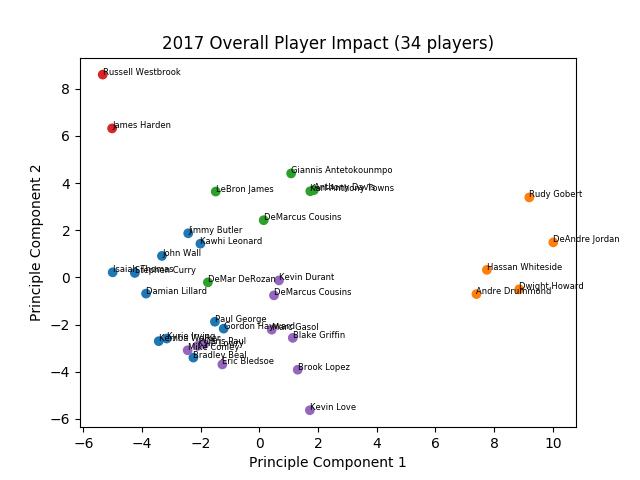
\includegraphics[width=9cm]{2017_Graphs/PCA_Overall_2017.png}
  \caption{PCA + kMeans of 2017 NBA players.}
\end{figure}

Through experimentation with different values of the hyperparameter, it was determined that $k=5$ was a suitable value for the number of desired clusters in the kMeans algorithm (the error plot is shown in Figure 3 below). From these results, a few important trends become evident. The first is that the algorithm does a good job of clustering "similar" players together. In the plot, a number of these groups match emprical observation. For instance, the orange cluster to the right of the graph clusters together many of the league's most dominant big men (such as Rudy Gobert, DeAndre Jordan, and Hassan Whiteside), who are reknowned for their rebounding and defensive capabilities. In contrast, the blue cluster towards the left puts together some of the league's high usage ball-dominant point guards (including Stephen Curry, Kyrie Irving, and Isaiah Thomas). The green cluster puts together some of the league's best skilled forwards (such as LeBron James, Giannis Antetokounmpo, and Anthony Davis), while the purple cluster groups together lesser skilled players (like Brook Lopez and Eric Bledsoe). 

Interestingly, the red cluster includes only Russell Westbrook and James Harden, the two leading candidates for MVP in the 2017 season, isolated far in the upper left corner. This suggests that they were simply on another level of ball-dominance and high usage production in this season, compared to their peers. In general, a player in a cluster as far from other players is demonstrative of high value. Unfortunately, the current construction of the model does not standardize the principal components so that the most valuable players are consistently in one section of the plot, but as this is simply a tool for justifying our MVP prediction, it provides a good way of visualizing impact as compared to other players. As such, we see that since Westbrook is the furthest to the upper left of the graph, there is strong evidence for him deserving the award over James Harden and other players in the league that season.

\begin{figure}[h]
  \centering
  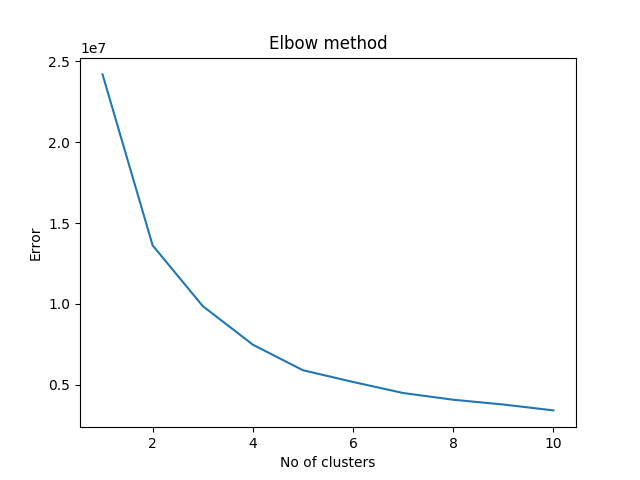
\includegraphics[width=9cm]{2017_Graphs/K_Means_Error_2017.png}
  \caption{kMeans error plot for 2017 player data.}
\end{figure}

\newpage Additionally, the model was applied to 5 other previous NBA seasons, producing the graphs shown below:

\begin{figure}[h]
  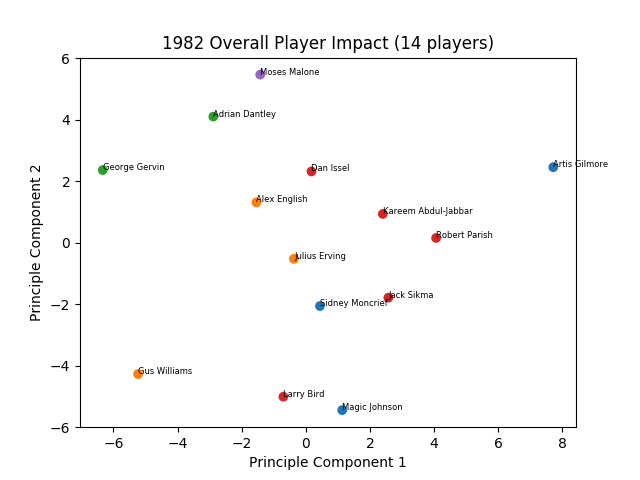
\includegraphics[width=7cm]{1982_Graphs/PCA_Overall_1982.png}
  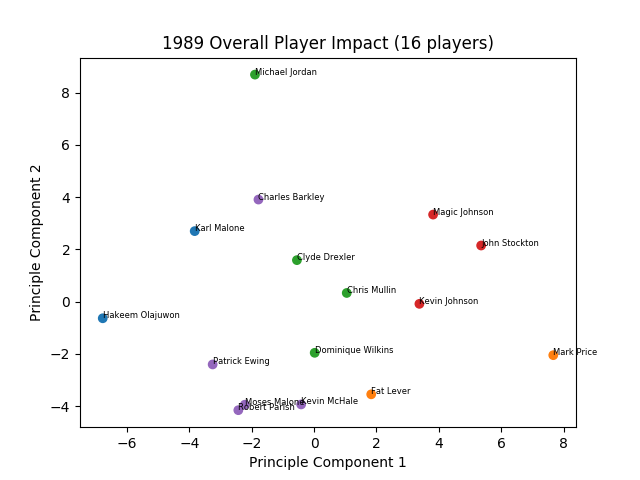
\includegraphics[width=7cm]{1989_Graphs/PCA_Overall_1989.png}
  \caption{PCA + kMeans of 1982 and 1989 NBA players.}
\end{figure}

\begin{figure}[h]
  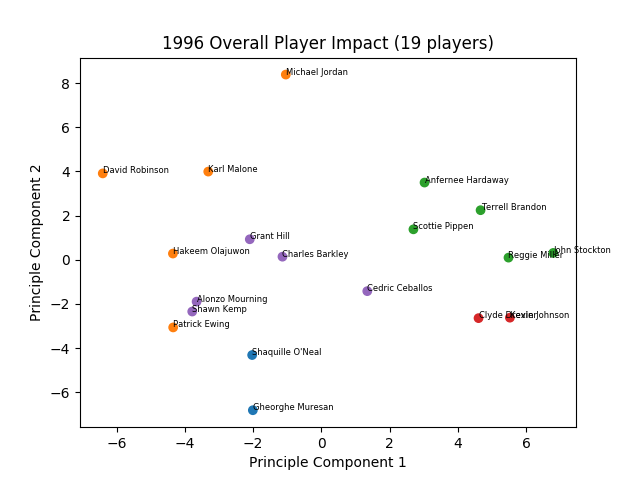
\includegraphics[width=7cm]{1996_Graphs/PCA_Overall_1996.png}
  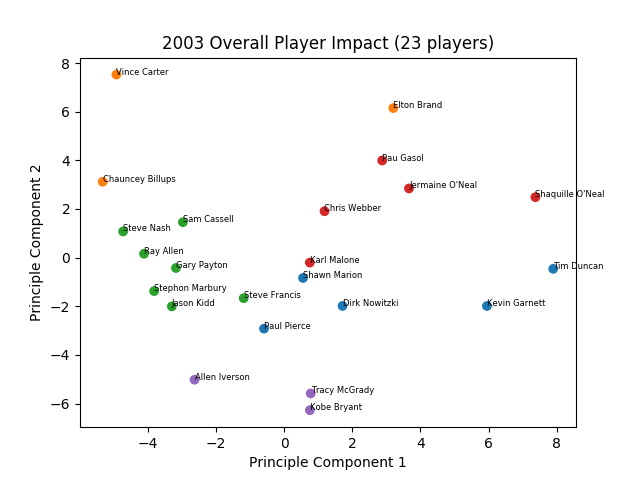
\includegraphics[width=7cm]{2003_Graphs/PCA_Overall_2003.png}
  \caption{PCA + kMeans of 1996 and 2003 NBA players.}
\end{figure}

\begin{figure}[h]
  \centering
  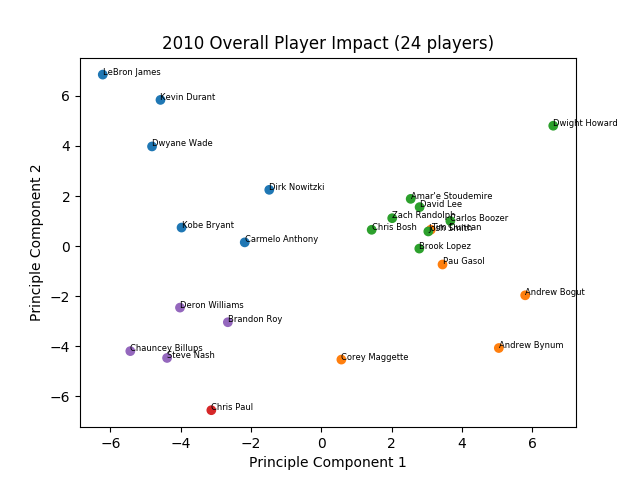
\includegraphics[width=7cm]{2010_Graphs/PCA_Overall_2010.png}
  \caption{PCA + kMeans of 2010 NBA players.}
\end{figure}

\newpage In these seasons, we also see that the model performed well in separating different types of players (big men, skilled wings, point guards, etc.) The MVPs of each of these seasons were: 

\begin{itemize}
  \item 1982 - Moses Malone
  \item 1989 - Magic Johnson
  \item 1996 - Michael Jordan
  \item 2003 - Tim Duncan
  \item 2010 - LeBron James
\end{itemize}

Interestingly, in each of these seasons aside from 1989, the MVP of the season was considerably farther isolated from his peers (towards the top of each plot), suggesting that the model does indeed do a good job of quantifying player value regardless of the time period. In addition, for 1989, the model isolates Michael Jordan towards the top of the graph. That year's MVP race was heavily debated between Michael Jordan and Magic Johnson, who won the award. This data suggests that perhaps Jordan should have won the award over Johnson, given how much more of an impact the plot shows he had as compared to his peers.

\subsubsection{Offensive Impact}

For the 2017 data, solely offensive features were also examined, in order to gauge just the offensive impact of NBA players. Again, $k=5$ was determined to be a suitable value of the hyperparameter. The results are shown below:

\begin{figure}[h]
  \centering
  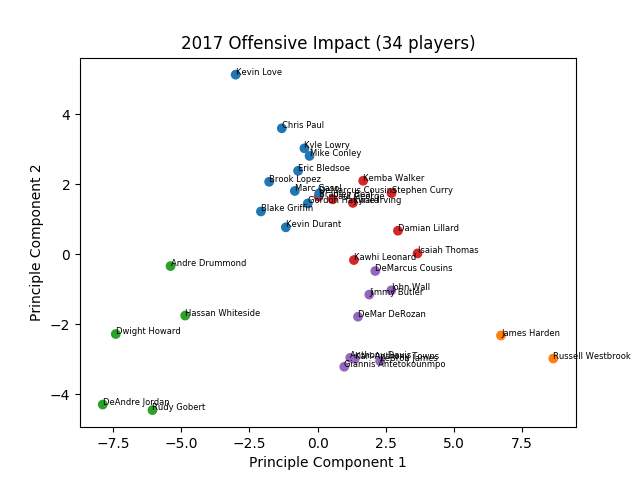
\includegraphics[width=9cm]{2017_Graphs/PCA_2017_Offensive.png}
  \caption{PCA + kMeans of 2017 NBA players (offensive features only).}
\end{figure}

From this, we see that the model again does a good job of gauging offensive value, as players of similar offensive skill sets are grouped together very similarly. Again, Westbrook and Harden are in a cluster of their own, showing that their value came in large part due to their offensive prowess.

\subsubsection{Defensive Impact}

Similarly, in 2017, defensive features were isolated, in order to gauge similarities in elite NBA players' defensive impact. However, for defensive features, after testing many values of the hyperparameter $k$, it was determined that no $k$ value performed suitably well in clustering the data points according to player similarity. The graphs below show the results of the model for a few $k$ values:

\begin{figure}[h]
  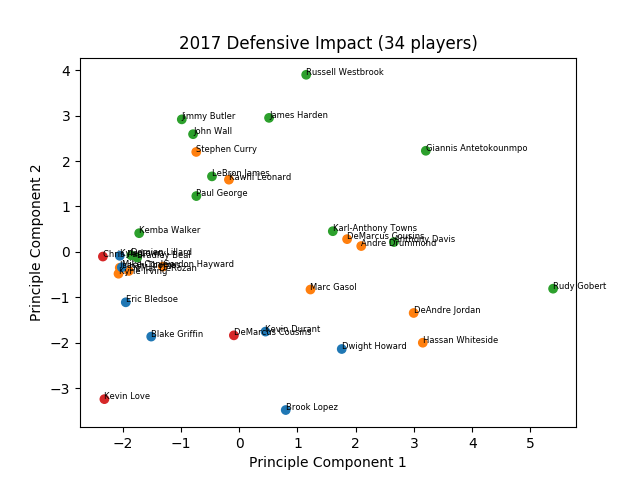
\includegraphics[width=7cm]{2017_Graphs/PCA_2017_Defensive_4.png}
  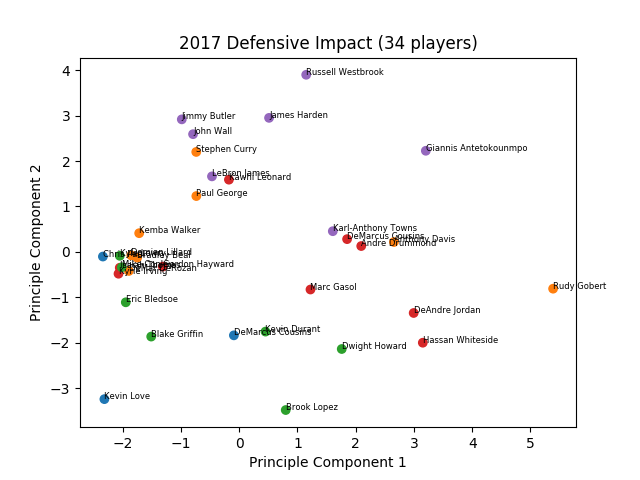
\includegraphics[width=7cm]{2017_Graphs/PCA_2017_Defensive_5.png}
  \caption{PCA + kMeans of 2017 NBA players (defensive features only; k = 4, 5).}
\end{figure}

\begin{figure}[h]
  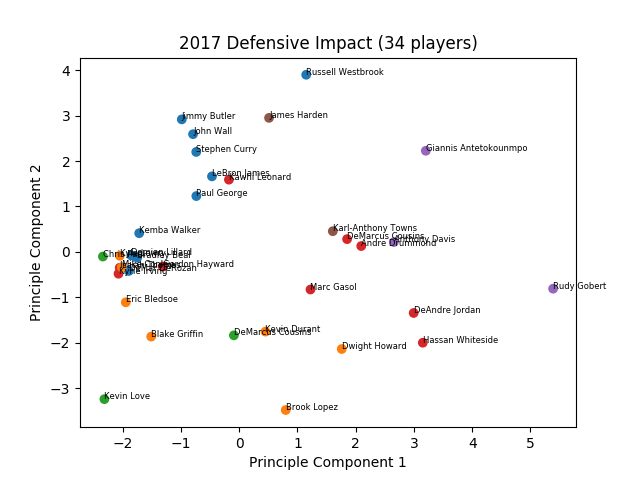
\includegraphics[width=7cm]{2017_Graphs/PCA_2017_Defensive_6.png}
  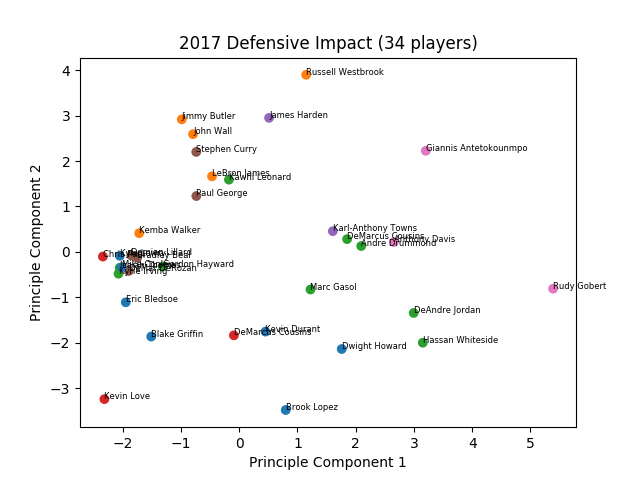
\includegraphics[width=7cm]{2017_Graphs/PCA_2017_Defensive_7.png}
  \caption{PCA + kMeans of 2017 NBA players (defensive features only; k = 6, 7).}
\end{figure}

\begin{figure}[h]
  \centering
  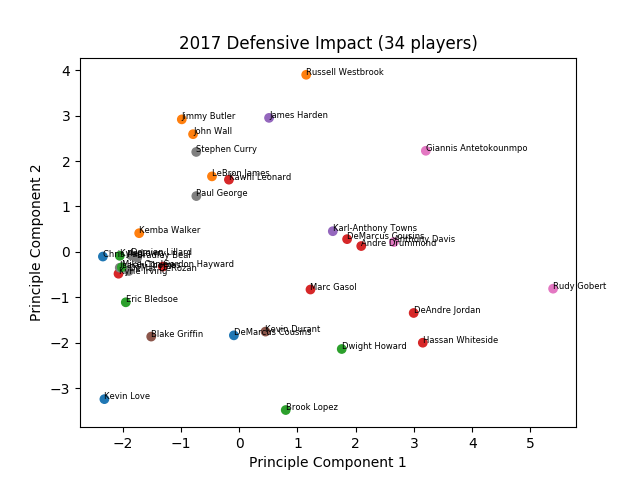
\includegraphics[width=7cm]{2017_Graphs/PCA_2017_Defensive_8.png}
  \caption{PCA + kMeans of 2017 NBA players (defensive features only; k = 8).}
\end{figure}

From these graphs, it is evident that kMeans clustering is largely ineffecttive on the defensive statistics data. This is likely reflective of the fact that in general, defensive statistics do a poor job of quantifying a player's defensive impact. Statistics like steals and blocks are limited in scope, and do not account for consistent defensive value throughout an entire game, but rather particular moments of defensive skill. As a result, the model performs poorly and not much can be inferred from these results.

\subsection{Drawbacks}

The dataset itself had some drawbacks that were reflected in the model. For instance, the dataset did not factor in team success throughout the regular season (how many games a given player's team won). This is generally a very relevant factor to the MVP discussion, as good players putting up good numbers on a bad team is not considered as valuable as a good player leading his team to a high win-total. While it does incorporate the variable of win-shares, a metric designed to capture some aspects of team success, this is not a complete picture of team success, as it is not always correlated to total team wins. This may have influenced the model's choice of Russell Westbrook over James Harden in the aforementioned 2017 race, as the main argument for Harden was that he led his team to more wins than Westbrook did that season. Perhaps James Harden really did deserve the award, and running this model on a dataset that factored in more team statistics would reveal that. Also, the dataset is not completely up-to-date, as it only goes up to 2017, missing out on the data of the previous 3 seasons. A more up-to-date dataset might alter the model in terms of which criteria it values more. It's also important to note that while the data provides full summary statistics, historically defensive skills are not well-captured by these statistics, which the NBA itself has admitted. Thus, the model likely under accounts for defense when assessing MVP, and explains why many of the top players it named were mainly offensive-minded players.

Additionally, the model developed had drawbacks that could certainly be improved upon. While the model was able to accurately predict the winner and runner-up for the award in 2017, it was not able to give a very accurate picture of the MVP race that season beyond those two players. One factor that was noticeable was the fact that the model tended to overrate so-called "big men". These are Centers and Power Forwards, some of the largest and tallest players on the court, that typically dominate stats such as Rebounds and Blocks. However, the way that the game is structured, these players aren't inherently more valuable than smaller players, as they often possess very different skill sets. Of the top 20 players list referenced earlier, 9 out of the 10 players that weren't named All-Stars were big men. A reason for this could be that throughout the early NBA, many big men dominated the league and won a great number of MVPs, which could have skewed the model into overvaluing stats typically dominated by bigger players, such as Field Goal Percentage and Rebounds. However, over time, the league has evolved to value smaller players with skills such as 3 point shooting and playmaking, resulting in the discrepancy.

\section{\Large Future Research Topics}

There are many possibilities for future research in this area. The currently existing model can certainly be improved in many ways. First and foremost, the logistic regression approach could be improved somewhat by better feature selection and scaling, as the large number of features may have contributed to some of the variability. Cross-validation could also be performed to improve on generalization error. The problem of not accounting for time-dependence of data could be remedied by testing the model on subsets of the given data, to account for different eras of basketball (such as the 2000s onwards or the 2010s onwards). Additionally, we could take a different approach to model the data. For example, a neural network model might produce a more accurate picture of player rankings. There are also many other interesting questions in the area of basketball analytics that can be answered by this dataset and related datasets. For example, a similar approach could be taken to predict All-Stars or All-NBA team selections.  Additional research can also be done on analyzing the correlation of different player types found by the kMeans approach and player salary data to determine if players' contracts are appropriately valued. Lastly, the deficiency of the model to examine player similarity on the defensive end suggests new avenues of research on that end. Formulating more consistent defensive metrics that do a better job of quantifying a single player's impact is an area of research that can certainly be pursued, perhaps through a visual analysis of players on a court.

\section*{References}


[1] Goldstein, Omri. "NBA Players Stats since 1950." {\it Kaggle}, 27 Apr. 2018, www.kaggle.com\/drgilermo\/nba-players-stats\#Seasons\_Stats.csv.

[2] Levene, Jake, and Zach Diamandis. "NBA MVP Predictions." {\it The Harvard Sports Analysis Collective}, 19 June 2018, harvardsportsanalysis.org\/2018\/06\/nba\-mvp\-predictions\/.

[3] Li, Peter. "NBA MVP Prediction Model." {\it Medium}, Towards Data Science, 20 Apr. 2019, towardsdatascience.com\/nba\-mvp\-predictor\-c700e50e0917.

[4] "Lloyd's Algorithm." {\it Wikipedia}, Wikimedia Foundation, 6 Mar. 2020, en.wikipedia.org/wiki/Lloyd%27s_algorithm.

\end{document}